\chapter{Stiefel-Whitney Classes}\label{ch-4}

This section will begin the study of characteristic classes by 
introducing four axioms which characterize the Stiefel-Whitney cohomology
classes of a vector bundle. The existence and uniqueness of cohomology
classes satisfying these axioms will only be established in later sections.

The expression $\homology^i(\B ; G)$ denotes the $i$-th singular cohomology group
of $\B $ with coefficients in $G$. For an outline of basic definitions and
theorems concerning singular cohomology theory, the reader is referred to
\Cref{app-A}. In this section the coefficient group will always be $\Z/2$,
the group of integers modulo $2$.

\noindent\textbf{\textsf{AXIOM 1.}} To each vector bundle $\xi$ there corresponds a sequence of
cohomology classes
\[w_i(\xi)\in\homology^i(\B (\xi); \Z/2),\quad i=0,1,2,\dots, \]
called the \textit{Stiefel-Whitney classes} of $\xi$. The class $w_0(\xi)$ is equal to
the unit element
\[1\in\homology^0(\B (\xi); \Z/2),\]
and $w_i(\xi)$ equals zero for $i$ greater than $n$ if $\xi$ is an $n$-plane bundle.
\vspace{.25cm}

\noindent\textsf{\textbf{AXIOM 2.}} \textsc{(Naturally)}. If $\map{f}{\B (\xi)}{\B (\xi)}$  is covered by a bundle
map from $\xi$ to $\eta$, then
\[w_i(\xi)=f^*w_i(\eta).\]
\vspace{.25cm}

\noindent\textsf{\textbf{AXIOM 3.}} \textsc{(The Whitney product Theorem).} If $\xi$  and  $\eta$ are
vector bundles over the same base space, then
\[w_k(\xi\oplus\eta)=\sum_{i=0}^kw_i(\xi)\smile w_{k-i}(\eta). \]
For example
\begin{align*}
		w_{1}(\xi \oplus \eta)&=w_{1}(\xi)+w_{1}(\eta) \\
		w_{2}(\xi \oplus \eta)&=w_{2}(\xi)+w_{1}(\xi) w_{1}(\eta)+w_{2}(\eta), \text { etc.}
\end{align*}
(We will omit the symbol $\smile$ for cup product whenever it seems convenient.)
\vspace{.25cm}

\noindent\textsf{\textbf{AXIOM 4.}} For the line bundle $\gamma^1_1$ over the circle $\rp{1}$, the Stiefel-
Whitney class $w_1(\gamma^1_1)$ is non-zero.
\begin{remark*}
	Characteristic \textit{homology} classes for the tangent bundle of
	a smooth manifold were defined by Stiefel in 1935 \cite{53}. In the same year
	Whitney defined the classes $w_i$ for any sphere bundle over a simplicial
	complex \cite{48}. (A ``sphere bundle" is the object obtained from a Euclidean
	vector bundle by considering only vectors of unit length in the total space.)
	The Whitney product theorem is due to Whitney, \cite{49,50} and Wu, \cite{55}. This axiomatic definition of Stiefel-Whitney classes was suggested
	by Hirzebruch, \cite[p.~58]{54}, where an analogous definition of Chern
	classes is given.
\end{remark*}

It is not at all obvious that classes $w_i(\xi)$ satisfying the four axioms
can be defined. Nevertheless this will be assumed for the rest of \S 4. A
number of applications of this assumption will be given.

\subsection*{Consequences of the Four Axioms}
As immediate consequences of Axiom 2 one has the following.
\begin{proposition}\label{prop-4-1}
	If $\xi$ is isomorphic to $\eta$ then $w_i(\xi)=w_i(\eta)$.
\end{proposition}
\begin{proposition}\label{prop-4-2}
If $\mathcal{E}$ is a trivial vector bundle then $w_i(\mathcal{E})=0$ for $i>0$.
\end{proposition}

For if $\mathcal{E}$ is trivial then there exists a bundle map from $\mathcal{E}$ to a vector
bundle over a point.


Combining this information with the Whitney product theorem, one 
obtains:

\begin{proposition}\label{prop-4-3}
If $\mathcal{E}$ is a trivial, then $w_i(\mathcal{E}\oplus\eta)=w_i(\eta)$.
\end{proposition}
\begin{proposition}\label{prop-4-4}
If $\xi$ is an $\R^n$-bundle with a Euclidean metric
which possesses a nowhere zero cross-section, then $w_n(\xi) = 0$.
If $\xi$ possesses $k$ cross-sections which are nowhere linearly
dependent, then
\[w_{n-k+1}(\xi)=w_{n-k+2}(\xi)=\dots=w_{n}(\xi)=0.\]
\end{proposition}

For it follows from \cref{thm-3-3} that $\xi$ splits as a Whitney sum
$\mathcal{E}\oplus\mathcal{E}^\perp$ where $\mathcal{E}$ is trivial and $\mathcal{E}^\perp$ has dimension $n-k$.

A particularly interesting case of the Whitney product theorem occurs
when the Whitney sum $\xi\oplus\eta$ is trivial. Then the relations
\begin{align*}
		&w_{1}(\xi)+w_{1}(\eta)=0 \\
		&w_{2}(\xi)+w_{1}(\xi) w_{1}(\eta)+w_{2}(\eta)=0 \\
		&w_{3}(\xi)+w_{2}(\xi) w_{1}(\eta)+w_{1}(\xi) w_{2}(\eta)+w_{3}(\eta)=0, \text { etc. }
\end{align*}
can be solved inductively, so that $w_i(\eta)$ is expressed as a polynomial
in the Stiefel-Whitney classes of $\xi$. It is convenient to introduce the 
following formalism.
\begin{definition}\label{def:4-1}
	$\homology^{\Pi}(\mathcal{\B };\Z/2)$ will denote the ring consisting of all 
	formal infinite series
	\[a=a_0+a_1+a_2+\cdots \]
	with $a_i\in\homology^i(\B ;\Z/2)$. The product operation in this ring is to be given
	by the formula 
\begin{align*}
	\left(a_{0}+a_{1}+a_{2}+\cdots\right)\left(b_{0}+b_{1}+b_{2}+\cdots\right)=\left(a_{0} b_{0}\right)&+\left(a_{1} b_{0}+a_{0} b_{1}\right)\\&+\left(a_{2} b_{0}+a_{1} b_{1}+a_0b_2\right)+\cdots\ .
\end{align*}
	This product is 
	commutative (since we are working modulo $2$) and associative. Additively,  
	$\homology^{\Pi}(\B ;\Z/2)$ is to be simply the Cartesian product of the groups $\homology^i(\B ;\Z/2)$.
	
	The \textit{total Stiefel-Whitney class} of an $n$-plane bundle $\xi$ over $\B $ is
	defined to be the element
	\[w(\xi)=1+w_{1}(\xi)+w_{2}(\xi)+\dots+w_{n}(\xi)+0+\cdots\]
	of this ring. Note that the Whitney product theorem can now be expressed
	by the simple formula
	\[w(\xi \oplus \eta)=w(\xi) w(\eta).\]
\end{definition}

\begin{lemma}\label{lem-4-1}
	The collection of all infinite series
	\[w=1+w_1+w_2+\cdots\quad\in\homology^{\Pi}(\B ;\Z/2)\]
	with leading term $1$ forms a commutative group under 
	multiplication.
\end{lemma}
(This is precisely the group of units of the  ring $\homology^{\Pi}(\B ;\Z/2)$.)

\begin{proof}
	The inverse
	\[\bar{w}=1+\bar{w}_{1}+\bar{w}_{2}+\bar{w}_{3}+\cdots\]
	of a given element $w$ can be constructed inductively by the algorithm
		\[\bar{w}_{n}=w_{1} \bar{w}_{n-1}+w_{2} \bar{w}_{n-2}+\dots+w_{n-1}\bar{w}_{1}+w_{n}\]
	Thus one obtains:
	\begin{align*}
		\bar{w}_{1}&=w_{1}, \\
		\bar{w}_{2}&=w_{1}^{2}+w_{2}, \\
		\bar{w}_{3}&=w_{1}^{3}+w_{3},\\
		\bar{w}_{4}&=w_{1}^{4}+w_{1}^{2} w_{2}+w_{2}^{2}+w_{4},
	\end{align*}
	and so on. This completes the proof.
\end{proof}

Alternatively $\bar{w}$ can be computed by the power series expansion:
\begin{align*}
	\bar{w}=&\left[1+\left(w_{1}+w_{2}+w_{3}+\cdots\right)\right]^{-1} \\
	=& 1-\left(w_{1}+w_{2}+w_{3}+\cdots\right)+\left(w_{1}+w_{2}+w_{3}+\cdots\right)^{2} \\
	&\phantom{1} -\left(w_{1}+w_{2}+w_{3}+\cdots\right)^{3}+-\cdots \\
	=& 1-w_{1}+\left(w_{1}^{2}-w_{2}\right)+\left(-w_{1}^{3}+2 w_{1} w_{2}-w_{3}\right)+\cdots
\end{align*}
(where the signs are of course irrelevant). This leads to the precise expression $(i_1+\dots+i_k)/i_1!\dotsi_k!$ for the coefficient of $w_{1}^{i_{1}} w_{2}^{i_{2}} \cdots w_{k}^{i_{k}}$ in $\bar{w}$.

Now consider two vector bundles $\xi$ and $\eta$ over the same base space.
It follows from \cref{lem-4-1} that the equation
\[w(\xi \oplus \eta)=w(\xi) w(\eta),\]
can be uniquely solved as
\[w(\eta)=\bar{w}(\xi) w(\xi \oplus \eta).\]
In particular, if $\xi \oplus \eta$ is trivial, then
\[w(\eta)=\bar{w}(\xi).\]
One important special case is the following.
\begin{lemma}[Whitney duality theorem]\label{lem-4-2}
	If $\tau_M$ is the tangent
	bundle of a manifold in Euclidean space and $\nu$ is the normal
	bundle then
	\[w_i(\nu)=\bar{w}(\tau_M).\]
\end{lemma}
Now let us compute the Stiefel-Whitney classes in some special cases.
It will frequently be convenient to use the abbreviation w(M) for the total
Stiefel-Whitney class of a tangent bundle $\tau_M$.

\begin{example}\label{ex-4-1}
	For the tangent bundle $\tau$ of the unit sphere $\Sphere{n}$, the class
	$w(\tau) =w(\Sphere{n})$ is equal to $1$. In other words, $\tau$ cannot be distinguished
	from the trivial bundle over $\Sphere{n}$ by means of Stiefel-Whitney classes.
	\begin{proof}
		For the standard imbedding $\Sphere{n}\subset\R^{n+1}$, the normal bundle $\nu$
		is trivial. Since $w(\tau)w(\nu) = 1$ and $w(\nu) = 1$ it follows that $w(\tau) = 1$.
	\end{proof}
\begin{proof}[Alternative proof (without using the Whitney product theorem)] The
	canonical map
	\[\map{f}{\Sphere{n}}{\rp{n}}\]
	to projective space is locally a diffeomorphism. Hence the induced map
		\[\map{\mathsf{D}f}{T\Sphere{n}}{T\rp{n}}\]
		of tangent bundles is a bundle map. Applying Axiom 2, one obtains the
		identity
		\[f^*w_n(\rp{n})=w_n(\Sphere{n});\]
		where the homomorphism
		\[\map{f^*}{\homology^n(\rp{n};\Z/2)}{\homology^n(\Sphere{n};\Z/2)}\]
		is well known to be zero. (Compare the remark below.) Therefore
		$w_n(\Sphere{n}) =0$, which completes the alternative proof. 
\end{proof}
\end{example}

The rest of \S 4 will be concerned with bundles over the projective
space $\rp{n}$. It is first necessary to describe the mod $2$ cohomology of $\rp{n}$.

\begin{lemma}\label{lem-4-3}
	The group $\homology^i(\rp{n};\Z/2)$ is cyclic of order $2$ for
	$0 \leq i \leq n$ and is zero for higher values of $i$. Furthermore, if
	$a$ denotes the non-zero element of $\homology^1(\rp{n};\Z/2)$ then each
	$\homology^i(\rp{n};\Z/2)$ is generated by the $i$-fold cup product $a^i$.
\end{lemma}

Thus $\homology^*(\rp{n};\Z/2)$ can be described as the algebra with unit over
$\Z/2$ having one generator a and one relation $a^{n+1} = 0$.

For a proof the reader may refer to \cite[\S~4.3.3]{56} or
\cite[p.~264]{57}. See \cref{prob-11-A} and \cref{prob-12-C}. (Compare 14.4.)

\begin{remark}
	This lemma can be used to compute the homomorphism
	\[f^*\mathpunct{:}\homology^n(\rp{n};\Z/2)\longrightarrow \homology^n(\Sphere{n};\Z/2)\]
	providing that $n > 1$. In fact
	\[f^*(a^n)=(f^*a)^n\]
	is zero since $f^{*}a \in \homology^{1}\left(\Sphere{n};\Z/2\right)=0$.
\end{remark}

\begin{example}\label{ex-4-2}
	The total Stiefel-Whitney class of the canonical line bundle $\gamma^{1}_{n}$ over $\rp{n}$ is given by
	\[w(\gamma^1_n)=1+a.\]
	\begin{proof}
	The standard inclusion $j\mathpunct{:} \rp{1}\rightarrow\rp{n}$ is clearly covered by a
	bundle map from $\gamma^1_1$ to $\gamma^1_n$. Therefore	
	\[j^*w_1(\gamma^1_n)=w_1(\gamma^1_1)\neq 0.\]
	This shows that $w_1(\gamma^1_n)$ cannot be zero, hence must be equal to $a$. Since
	the remaining Stiefel-Whitney classes of $\gamma^1_n$ are determined by Axiom 1,
	this completes the proof.
	\end{proof}
\end{example}
\begin{example}\label{ex-4-3}
	By its definition, the line bundle $\gamma^1_n$ over $\rp{n}$ is contained as a sub-bundle in the trivial bundle $\mathcal{E}^{n+1}$. Let $\gamma^\perp$ denote the orthogonal complement of $\gamma^1_n$ in $\mathcal{E}^{n+1}$.
	(Thus the total space $E(\gamma^\perp)$
	consists of all pairs \[(\{\pm x\}, v) \in \rp{n} \times \R^{n+1}\] with $v$ perpendicular to $x$.) Then
	\[w(\gamma^{\perp})=1+a+a^{2}+\dots+a^{n}.\]
\begin{proof}
	Since $\gamma_{n}^{1} \oplus \gamma^{\perp}$ is trivial we have
\[w(\gamma^{\perp})=\overline{w}(\gamma_{n}^{1})=(1+a)^{-1}=1+a+a^{2}+\dots+a^{n}.\qedhere\]
\end{proof}
\end{example}
This example shows that all of the $n$ Stiefel-Whitney classes of an
$\R^n$--bundle may be non-zero.

\begin{example}\label{ex-4-4}
Let $\tau$ be the tangent bundle of the projective space $\rp{n}$.	
\end{example}

\begin{lemma}\label{lem-4-4}
The tangent bundle $\tau$ of $\rp{n}$ is isomorphic to
$\Hom (\gamma^1_n,\gamma^1)$.	
\end{lemma}
\begin{proof}
	Let $L$ be a line through the origin in $\R^{n+1}$, intersecting $\Sphere{n}$
	in the points $\pm x$, and let $L^\perp\subset \R^{n+1}$ be the complementary $n$--plane. Let
	$f\colon \Sphere{n}\to \rp{n}$ denote the canonical map, $f(x) =
	\{\pm x\}$. Note that the two 
	tangent vectors $(x, v)$ and $(-x, -v)$ in $\mathsf{D}\Sphere{n}$ both have the same image
	under the map
	\[\map{\mathsf{D}f}{\mathsf{D}\Sphere{n}}{\mathsf{D}\Sphere{n}}\]
	which is induced by $f$. (Compare \cref{fig5}.) Thus the tangent manifold
	$\mathsf{D}\rp{n}$ can be identified with the set of all pairs $\{(x, v), (-x, -
		v)\}$ 
		satisfying
	\[x\cdot x=1,\qquad x \cdot v=0. \]
	But each such pair determines, and is determined by, a linear mapping
	\[\map{\ell}{L}{L^\perp},\]
	where $\ell(x)=v$. Thus the tangent space of $\rp{n}$ at $\{\pm x\}$ is canonically isomorphic to the
		vector space $\Hom (L, L^\perp)$. It follows that the tangent vector bundle $\tau$ is canonically isomorphic to the bundle $\Hom (\gamma^1_n,\gamma^1)$. This completes
		the proof of \cref{lem-4-4}. 
\end{proof}
\begin{figure}[!htb]
	\centering\includegraphics[scale=.8]{fig5}
	\caption{}\label{fig5}
\end{figure}

We cannot compute $\omega(\rp{n})$ directly from this lemma since we do not
yet have any procedure for relating the Stiefel-Whitney classes of
$\Hom (\gamma^1_n,\gamma^1)$ to those of $\gamma^1_n$ and $\gamma^1$. However the computation can be
carried through as follows. Let $\mathcal{E}^1$ be a trivial line bundle over $\rp{n}$.

\begin{theorem}\label{thm-4-5}
The Whitney sum $\tau \oplus \mathcal{E}^1$ is isomorphic to the
$(n+1)$-fold Whitney sum $\gamma_{n}^{1} \oplus \gamma_{n}^{1} \oplus \dots \oplus \gamma_{n}^{1}$. Hence the total
Stiefel-Whitney class of $\rp{n}$ is given by
\[
w\left(\rp{n}\right)=(1+a)^{n+1}=1+\binom{n+1}{1} a+\binom{n+1}{2} a^{2}+\dots+\binom{n+1}{n} a^{n}
\]	
\end{theorem}
\begin{proof}
	The bundle $\Hom (\gamma^1_n,\gamma^1)$ is trivial since it is a line bundle
	with a canonical nowhere zero cross-section. Therefore
	\[\tau \oplus \mathcal{E}^1\cong \Hom (\gamma^1_n,\gamma^\perp)\oplus \Hom (\gamma^1_n,\gamma^1_n). \]
	This is clearly isomorphic to
	\[ \Hom (\gamma^1_n,\gamma^\perp\oplus\gamma^1_n)\cong \Hom (\gamma^1_n,\mathcal{E}^1), \]
	and therefore is isomorphic to the $(n+l)$-fold sum
	\[ \Hom (\gamma^1_n,\mathcal{E}^1\oplus\dots\oplus \mathcal{E}^1)\cong \Hom (\gamma^1_n,\mathcal{E}^1)\oplus\dots\oplus\Hom (\gamma^1_n,\mathcal{E}^1). \]
	But the bundle $\Hom (\gamma^1_n,\mathcal{E}^1)$ is isomorphic to $\gamma^1_n$, since $\gamma^1_n$ has a
	Euclidean metric. (Compare \cref{prob-3-D}.) This proves that
	\[\tau\oplus\mathcal{E}^1\cong \gamma_{n}^{1} \oplus \dots \oplus \gamma_{n}^{1}.\]
	Now the Whitney product theorem implies that $w(\tau)=w(\tau\oplus\mathcal{E}^1)$
	\[w(\gamma_{n}^{1}) \dots w(\gamma_{n}^{1})=(1+a)^{n+1}\]
	Expanding by the binomial theorem, this completes the proof of \cref{thm-4-5}.
\end{proof}

Here is a table of the binomial coefficients $\binom{n+1}{i}$ modulo $2$, for
$n\leq 14$.\\

\begin{figure}[!htb]
	\centering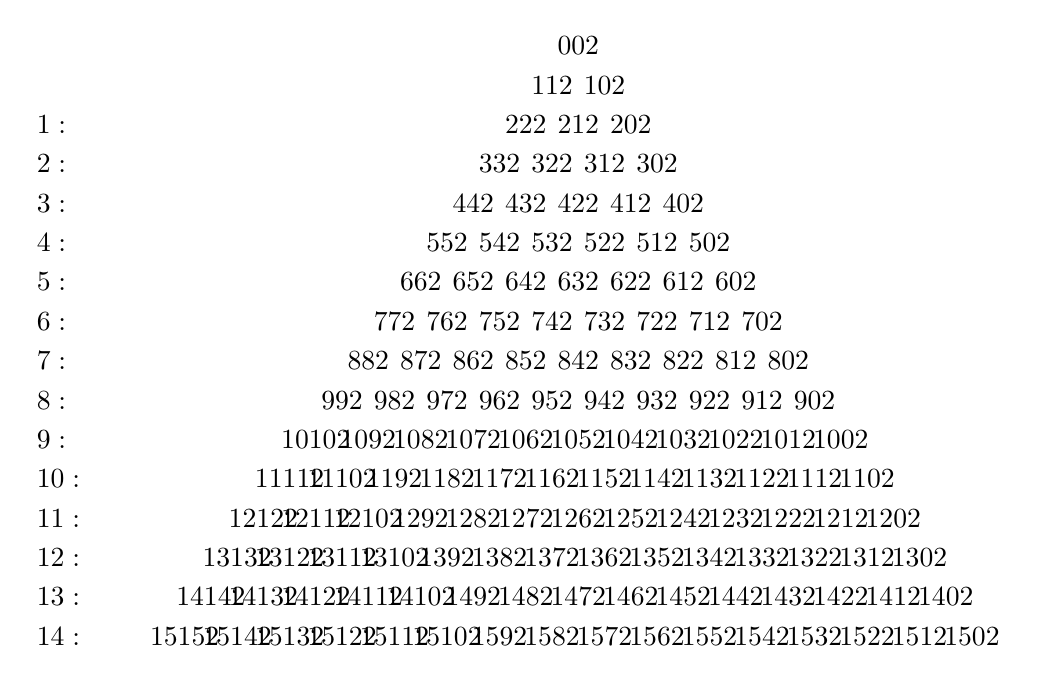
\begin{tikzpicture}[scale=1]
		\foreach \n in {0,...,15} {
			\foreach \k in {0,...,\n} {
				%				\node at (-7,-\n/2) {$n=\n$};
				\node at (-2*\k/3+\n/3,-\n/2) {\modulo{\binomialb\n\k}{2}};
			}
		}
		\foreach \n in {1,...,14} {
			\node[anchor=west] at (-7,-\n/2-1/2) {$\rp{\n}:$};}
	\end{tikzpicture}
\end{figure}



The right hand edge of this triangle can be ignored for our purposes
since $\homology^{n+1}(\rp{n}; \Z/2) = 0$. As examples one has:
\begin{align*}
	&w(\rp{2})=1+a+a^{2} \\
	&w(\rp{3})=1 \\ \intertext{and}
	&w(\rp{4})=1+a+a^{4}.
\end{align*}

\begin{corollary}[Stiefel]\label{cor-4-6}
	The class $w(\rp{n})$ is equal to $1$ if
	and only if $n + 1$ is a power of $2$. Thus the only projective
	spaces which can be parallelizable are $\rp{1}$, $\rp{3}$, $ \rp{7} $, $ \rp{15}, \dots\ $.
\end{corollary}

(We will see in a moment that $\rp{1},$ $\rp{3}$  and $ \rp{7} $ actually are 
parallelizable. On the other hand it is known that the higher projective spaces
$\rp{15}$, $\rp{31}$, $\dots$ are not parallelizable. See \cite{58,59,60}.)


\begin{proof}
The identity $(a + b)^2 \equiv
a^2 + b^2$ modulo $2$ implies that
$$
(1+a)^{2^{r}}=1+a^{2^{r}}
$$
Therefore if  $n+1=2^{r}$ then
\[
w(\rp{n})=(1+a)^{n+1}=1+a^{n+1}=1
\]
Conversely if $n+1=2^{r} m$ with $m$ odd, $m>1$, then
\begin{align*}
	w(\rp{n}) &=(1+a)^{n+1}=\left(1+a^{2^{r}}\right)^{m} \\
	&=1+m a^{2^{r}}+\frac{m(m-1)}{2} a^{2 \cdot 2^{r}}+\dots \neq 1
\end{align*}	
since $2^r < n + 1$. This completes the proof,
\end{proof}

\subsection*{Division algebras}

Closely related is the question of the existence of real division 
algebras.

\begin{theorem}[Stiefel]\label{thm-4-7}
Suppose that there exists a bilinear
product operation\footnote{This product operation is not required to be associative, or to have an
	identity element.}
\[\map{p}{\R^n\times\R^n}{\R^n} \]
without zero divisors. Then the projective space $\rp{n-1}$
is
parallelizable, hence $n$ must be a power of $2$.
\end{theorem}

In fact such division algebras are known to exist for $n =
1, 2, 4, 8$:
namely the real numbers, the complex numbers, the quaternions, and the
Cayley numbers. It follows that the projective spaces $\rp{1}, \rp{3}$ and $\rp{7}$
are parallelizable. That no such division algebra exists for $n > 8$ 
follows from the references cited above on parallelizability.	

\begin{proof}
Let $b_1,\dots, b_n$ be the standard basis for the vector
space $\R^n$. Note that the correspondence $y\mapsto p(y,b_1)$
defines an isomorphism of $\R^n$ onto itself. Hence the formula	
\[v_{i}\left(p(y, b_{1})\right)=p(y, b_{i}),\]
defines a linear transformation 
\[\map{v_i}{\R^n}{\R^n}.\]
Note that $v_{1}(x), \dots, v_{n}(x)$ are linearly independent for $x\neq 0$, and that
$v_1(x) = x$.

The functions $v_{2}, \dots, v_{n}$ give rise to $n-
1$ linearly independent
cross-sections of the vector bundle
\[\tau_{\rp{n-1}}\cong\Hom(\gamma^1_{n-1},\gamma^\perp).\]
In fact for each line $L$ through the origin, a linear transformation
\end{proof}

%==================================%mathpix

\[
\map{\overline{v}_{i}}{L}{L^{\perp}}
\]

is defined as follows. For $x \in L$, let $\overline{v}_{i}(x)$ denote the image of $v_{i}(x)$ under the orthogonal projection

\[
\R^{n} \longrightarrow L^{\perp}.
\]
Clearly $\overline{v}_{1}=0$, but $\overline{v}_{2}, \dots, \overline{v}_{n}$ are everywhere linearly independent. Thus the tangent bundle $\tau_{\rp{n-1}}$ is a trivial bundle. This completes the proof of \cref{thm-4-7}.

\subsection*{Immersions}

As a final application of \cref{thm-4-5}, let us ask which projective spaces can be immersed in the Euclidean space of a given dimension.

If a manifold $M$ of dimension $n$ can be immersed in the Euclidean space $\R^{n+k}$ then the Whitney duality theorem
\[
w_{i}(\nu)=\overline{w}_{i}(M)
\]
implies that the dual Stiefel-Whitney classes $\overline{w}_{i}(M)$ are zero for $i>k$.

As a typical example, consider the real projective space $\rp{9}$. Since
\[
w(\rp{9}):=(1+a)^{10}=1+a^{2}+a^{8}
\]
we have
\[
\overline{w}(\rp{9})=1+\mathrm{a}^{2}+\mathrm{a}^{4}+\mathrm{a}^{6}
\]
Thus if $\rp{9}$ can be immersed in $\R^{9+k}$, then $k$ must be at least $6$.

The most striking results for $\rp{n}$ are obtained when $n$ is a power of $2$. If $n=2^{r}$ then
\[
w(\rp{n})=(1+a)^{n+1}:=1+a+a^{n}
\]
hence
\[
\overline{w}\left(\rp{n}\right)=1+a+a^{2}+\dots+a^{n-1}.
\]
Thus:
\begin{theorem}\label{thm-4-8}
	If $\rp{2^{r}}$ can be immersed in $\R^{2^{r}+k}$, then $k$ must be at least $2^{r}-1$.
\end{theorem}

On the other hand Whitney has proved that every smooth compact manifold of dimension $n>1$ can actually be immersed in $\R^{2 n-1}$. (Reference: \cite{61}.) Thus \cref{thm-4-8} provides a best possible estimate.

Note that estimates for other projective spaces follow from \cref{thm-4-8}. For example since $\rp{8}$ cannot be immersed in $\R^{14}$, it follows a fortiori that $\rp{9}$ cannot be immersed in $\R^{14}$. This duplicates the earlier estimate concerning $\rp{9}$. See \cite{62}.

An extensive and beautiful theory concerning immersions of manifolds has been developed by S. Smale and M. Hirsch. For further information the reader should consult \cite{63} and \cite{64}.

\subsection*{Stiefel-Whitney Numbers}

We will now describe a tool which allows us to compare certain Stiefel-Whitney classes of two different manifolds.

Let $M$ be a closed, possibly disconnected, smooth $ n $-dimensional manifold. Using mod $2$ coefficients, there is a unique fundamental homology class
\[
\mu_{M} \in \homology_{n}(M ; \Z / 2),
\]
(See \Cref{app-A}.) Hence for any cohomology class $v \in \homology^{n}(M ; \Z / 2)$, the \textit{Kronecker index}
\[
\left\langle  v, \mu_{M}\right\rangle \in \Z / 2,
\]
is defined. We will sometimes use the abbreviated notation $v[M]$ for this Kronecker index.

Let $r_{1}, \dots, r_{n}$ be non-negative integers with $r_{1}+2 r_{2}+\dots+n r_{n}=n$. Then corresponding to any vector bundle $\xi$ we can form the monomial

\[
w_{1}(\xi)^{r_{1}} \dots w_{n}(\xi)^{r_{n}}
\]
in $\homology^{n}(\mathrm{B}(\xi) ; \Z / 2) .$ In particular we can carry out this construction if $\xi$ is the tangent bundle of the manifold $M$.

\begin{definition}\label{def:4-2}
	The corresponding integer mod $2$
	\[
	\left\langle w_{1}\left(\tau_{M}\right)^{r_1} \dots w_{n}\left(\tau_{M}\right)^{r_n}, \mu_{M}\right\rangle,\quad \text{ or briefly }\quad{w}_{1}{ }^{r_1} \dots w_{n}{ }^{r_n}[M]
	\]
	is called the Stiefel-Whitney number of $M$ associated with the monomial $w_{1}{ }^{r_{1}} \dots w_{n}{ }^{r_n}$.
\end{definition}

In studying these numbers, we will be interested in the collection of all possible Stiefel-Whitney numbers for a given manifold. Thus two different manifolds $M$ and $M^{\prime}$ have the same Stiefel-Whitney numbers if 
\[w_{1}{ }^{r_{1}} \dots w_{n}{ }^{r_{n}} \left[M\right]=w_{1}{ }^{r_{1}} \dots w_{n} { }^{r_n}{\left[M^{\prime}\right]}\]
for every monomial ${w}_{1}{ }^{r_{1}} \dots w_{n}{ }^{r_n}$ of total dimension $n$. (Compare \S $6.6$ and \Cref{prob-6-D}.)

As an example, let us try to compute the Stiefel-Whitney numbers of the projective space $\rp{n}$ (which is about the only manifold we are able to handle at this point). Let $\tau$ denote the tangent bundle of $\rp{r}$. If $n$ is even, then the cohomology class $w_{n}(\tau)=(n+1) a^{n}$ is non-zero, and it follows that the Stiefel-Whitney number $w_{n}\left[\rp{n}\right]$ is non-zero. Similarly, since $w_{1}(f)=(n+1) a \neq 0$, it follows that $w_{1}{ }^{n}{ }^{n}\left[\rp{n}\right] \neq 0$. If $n$ is actually a power of $2$, then $w(\tau):=1+a+a^{n}$, and it follows that all other Stiefel-Whitney numbers of $\rp{n}$ are zero. In any case, even if $n$ is not a power of $2$, the remaining Stiefel-Whitney numbers can certainly be computed effectively as products of binomial coefficients.

On the other hand if $n$ is odd, say $n=2k-1$, then $w(\tau)=(1+a)^{2k} =$\linebreak$(1+a^{2})^{k}$, so it follows that $w_{j}(\tau)=0$ whenever $j$ is odd. Since every monomial of total dimension $2 k-1$ must contain a factor $w_{j}$ of odd dimension, it follows that all of the Stiefel-Whitney numbers of $\rp{2 k-1}$ are zero. This gives some indication of how much detail and structure this invariant overlooks.

The importance of Stiefel-Whitney numbers is indicated by the following theorem and its converse.
\begin{theorem}[Pontrjagin]\label{thm-4-9}
If $B$ is a smooth compact $(n+1)$-dimensional manifold with boundary equal to $M$ (compare \cref{ch-17}),
		then the Stiefel-Whitney numbers of $M$ are all zero.
\end{theorem}
\begin{proof}
	Let us denote the fundamental homology class of the pair by
	\[\mu_B\in\homology_{n+1}(B,M),\]
	the coefficient group $\Z/2$ being understood. Then the natural homomorphism
	\[\map{\partial}{\homology_{n+1}(\B ,M)}{\homology_{n}(M)}\]
	maps $\mu_\B $ to $ \mu_M $. (Compare Appendix A.) For any class $v\in \homology_{n}(M)$,
	note the identity
	\[\ip{v,\partial\mu_\B }=\ip{\delta_{v},\mu_\B },\]
	where $\delta$ denotes the natural homomorphism from $\homology^{n}(M)$ to $\homology^{n+1}(\B ,M)$.
	(There is no sign since we are working mod $2$.) Consider the tangent
	bundle $\tau_\B $ restricted to $M$, as well as the sub-bundle $\tau_M$. Choosing a
	Euclidean metric on $\tau_\B $, there is a unique outward normal vector field
	along $M$, spanning a trivial line bundle $\mathcal{E}^1$, and it follows that
	\[\tau_\B |_M\cong\tau_M\oplus\mathcal{E}^1.\]
	Hence the Stiefel-Whitney classes of $\tau_\B $, restricted to $M$, are precisely
	equal to the Stiefel-Whitney classes $w_j$ of $\tau_M$. Using the exact sequence
	\[\homology^n(\B )\xrightarrow{\quad \iota^*\quad}\homology^n(M)\xrightarrow{\quad \delta\quad} \homology^{n+1}(\B ,M)\]
	where $ \iota^* $ is the restriction homomorphism, it follows that
	\[\delta({w}_{1}{ }^{r_{1}} \dots w_{n}{ }^{r_n})=0,\]
	and therefore
	\[\ip{\delta({w}_{1}{ }^{r_{1}} \dots w_{n}{ }^{r_n}),\partial\mu_\B }=\ip{\delta({w}_{1}{ }^{r_{1}} \dots w_{n}{ }^{r_n}),\mu_\B }.\]
	Thus all Stiefel-Whitney numbers of $M$ are zero.
\end{proof}
The converse theorem, due to Thom, is much harder to prove.
\begin{theorem}[Thom]\label{thm-4-10}
	If all of the Stiefel-Whitney numbers
	of $M$ are zero, then $M$ can be realized as the boundary of some
	smooth compact manifold.
	
\end{theorem}

For proof, the reader is referred to \cite{65}.

For example the union of two disjoint copies of $M$, which certainly
has all Stiefel-Whitney numbers zero, is equal to the boundary of the
cylinder $M\times [0, 1]$. Similarly, the odd dimensional projective space
$\rp{2k-1}$ has all Stiefel-Whitney numbers zero. The reader may enjoy trying
to prove directly that $\rp{2k-1}$ is a boundary.

Now let us introduce the concept of ``cobordism class."

\begin{definition}\label{def:4-3}
Two smooth closed $n$-manifolds $M_1$ and $M_2$ belong
to the same unoriented cobordism class iff their disjoint union $M_1 \sqcup M_2$
is the boundary of a smooth compact $(n+1)$-dimensional manifold.	
\end{definition}
\begin{figure}[!htb]
	\centering\includegraphics[scale=.8]{fig6}
	%\caption{}\label{fig6}
\end{figure}
\cref{thm-4-9,thm-4-10} have the following important consequence.
\begin{corollary}\label{cor-4-11}
Two smooth closed $n$-manifolds belong to
the same cobordism class if and only if all of their corresponding
Stiefel-Whitney numbers are equal.	
\end{corollary}
\begin{proof}
	The proof is immediate.
\end{proof}

Here are five problems for the reader.
\begin{problem}\label{prob-4-A}
	Show that the Stiefel-Whitney classes of a Cartesian
	product are given by 
	\[w_k(\xi\times \eta)=\sum_{i=0}^k w_i(\xi)\times w_{k-i}(\eta).\]
\end{problem}\bigskip
\begin{problem}\label{prob-4-B}
	Prove the following theorem of Stiefel. If $n + 1 = 2rm$
	with $m$ odd, then there do not exist $2r$ vector fields on the projective
	space $\rp{n}$ which are everywhere linearly independent.\footnote{Compare \cite{53,67,68}.}
\end{problem}\bigskip
\begin{problem}\label{prob-4-C}
	A manifold $M$ is said to admit a field of tangent $k$-
	planes if its tangent bundle admits a sub-bundle of dimension $k$. Show
	that $\rp{n}$ admits a field of tangent $1$-planes if and only if $n$ is odd. Show
	that $\rp{4}$ and $\rp{6}$ do not admit fields of tangent $2$-planes.
\end{problem}\bigskip
\begin{problem}\label{prob-4-D}
	If the $n$-dimensional manifold $M$ can be immersed in
	$\R^{n+1}$ show that each $w_i(M)$ is equal to the $i$-fold cup product $w_1(M)^i$.
	If $\rp{n}$ can be immersed in $\R^{n+1}$ show that $n$ must be of the form
	$2^r-1$ or $2^r-2$.
\end{problem}\bigskip
\begin{problem}\label{prob-4-E}
	Show that the set $\varPi_n$ consisting of all unoriented
	cobordism classes of smooth closed $n$-manifolds can be made into an
	additive group. This \textit{cobordism group} $\mathcal{\varPi}_n$ is finite by \cref{cor-4-11}, and is
	clearly a module over $\Z/2$. Using the manifolds $\rp{2}\times\rp{2}$ and $\rp{4}$,
	show that $\varPi_4$ contains at least four distinct elements.
\end{problem}